%% LyX 2.0.5.1 created this file.  For more info, see http://www.lyx.org/.
%% Do not edit unless you really know what you are doing.
\documentclass{article}\usepackage{graphicx, color}
%% maxwidth is the original width if it is less than linewidth
%% otherwise use linewidth (to make sure the graphics do not exceed the margin)
\makeatletter
\def\maxwidth{ %
  \ifdim\Gin@nat@width>\linewidth
    \linewidth
  \else
    \Gin@nat@width
  \fi
}
\makeatother

\IfFileExists{upquote.sty}{\usepackage{upquote}}{}
\definecolor{fgcolor}{rgb}{0.2, 0.2, 0.2}
\newcommand{\hlnumber}[1]{\textcolor[rgb]{0,0,0}{#1}}%
\newcommand{\hlfunctioncall}[1]{\textcolor[rgb]{0.501960784313725,0,0.329411764705882}{\textbf{#1}}}%
\newcommand{\hlstring}[1]{\textcolor[rgb]{0.6,0.6,1}{#1}}%
\newcommand{\hlkeyword}[1]{\textcolor[rgb]{0,0,0}{\textbf{#1}}}%
\newcommand{\hlargument}[1]{\textcolor[rgb]{0.690196078431373,0.250980392156863,0.0196078431372549}{#1}}%
\newcommand{\hlcomment}[1]{\textcolor[rgb]{0.180392156862745,0.6,0.341176470588235}{#1}}%
\newcommand{\hlroxygencomment}[1]{\textcolor[rgb]{0.43921568627451,0.47843137254902,0.701960784313725}{#1}}%
\newcommand{\hlformalargs}[1]{\textcolor[rgb]{0.690196078431373,0.250980392156863,0.0196078431372549}{#1}}%
\newcommand{\hleqformalargs}[1]{\textcolor[rgb]{0.690196078431373,0.250980392156863,0.0196078431372549}{#1}}%
\newcommand{\hlassignement}[1]{\textcolor[rgb]{0,0,0}{\textbf{#1}}}%
\newcommand{\hlpackage}[1]{\textcolor[rgb]{0.588235294117647,0.709803921568627,0.145098039215686}{#1}}%
\newcommand{\hlslot}[1]{\textit{#1}}%
\newcommand{\hlsymbol}[1]{\textcolor[rgb]{0,0,0}{#1}}%
\newcommand{\hlprompt}[1]{\textcolor[rgb]{0.2,0.2,0.2}{#1}}%

\usepackage{framed}
\makeatletter
\newenvironment{kframe}{%
 \def\at@end@of@kframe{}%
 \ifinner\ifhmode%
  \def\at@end@of@kframe{\end{minipage}}%
  \begin{minipage}{\columnwidth}%
 \fi\fi%
 \def\FrameCommand##1{\hskip\@totalleftmargin \hskip-\fboxsep
 \colorbox{shadecolor}{##1}\hskip-\fboxsep
     % There is no \\@totalrightmargin, so:
     \hskip-\linewidth \hskip-\@totalleftmargin \hskip\columnwidth}%
 \MakeFramed {\advance\hsize-\width
   \@totalleftmargin\z@ \linewidth\hsize
   \@setminipage}}%
 {\par\unskip\endMakeFramed%
 \at@end@of@kframe}
\makeatother

\definecolor{shadecolor}{rgb}{.97, .97, .97}
\definecolor{messagecolor}{rgb}{0, 0, 0}
\definecolor{warningcolor}{rgb}{1, 0, 1}
\definecolor{errorcolor}{rgb}{1, 0, 0}
\newenvironment{knitrout}{}{} % an empty environment to be redefined in TeX

\usepackage{alltt}
\usepackage[sc]{mathpazo}
\usepackage{geometry}
\geometry{verbose,tmargin=2.5cm,bmargin=2.5cm,lmargin=2.5cm,rmargin=2.5cm}
\setcounter{secnumdepth}{2}
\setcounter{tocdepth}{2}
\usepackage{url}
\usepackage[unicode=true,pdfusetitle,
 bookmarks=true,bookmarksnumbered=true,bookmarksopen=true,bookmarksopenlevel=2,
 breaklinks=false,pdfborder={0 0 1},backref=false,colorlinks=false]
 {hyperref}
\hypersetup{
 pdfstartview={XYZ null null 1}}
\usepackage{breakurl}
\begin{document}





\title{Stat 2025- HW 7}
\author{Michael Discenza}

\maketitle

We know that we have a binary response variable, "chd," where 0 represents the absence and 1 the presence of coronary heart disease. Because the goal of this exercise is predicting the score of the 42 rows, we will try to minimize cv prediction error.

First we load the data and split it into training and test sets.
\begin{knitrout}
\definecolor{shadecolor}{rgb}{0.969, 0.969, 0.969}\color{fgcolor}\begin{kframe}
\begin{alltt}
SAH <- \hlfunctioncall{read.table}(\hlstring{"http://stat.columbia.edu/~madigan/W2025/data/SAHmissing.txt"}, header = TRUE, 
    sep = \hlstring{"\textbackslash{}t"})
SAH.training <- \hlfunctioncall{na.exclude}(SAH)
SAH.test <- SAH[421:462, ]
\end{alltt}
\end{kframe}
\end{knitrout}


Here we are not so focused on creating "predictive"good" models with low BICs or AICs, we are more focused on predictive power.  We don't have to be so concerned with making small models that are as well vetted as long as they predict well.  Nonetheless, we start by fitting a ful model and seeing which variables are statistically significant, or nearly so, and which variables are not particularly informative.  We drop the non particularly informative variables (alcohol and adiposity) and use the rest in the the modeling processes.
\begin{knitrout}
\definecolor{shadecolor}{rgb}{0.969, 0.969, 0.969}\color{fgcolor}\begin{kframe}
\begin{alltt}
m1 <- \hlfunctioncall{glm}(chd ~ ., data = SAH.training)
\hlfunctioncall{summary}(m1)
\end{alltt}
\begin{verbatim}
## 
## Call:
## glm(formula = chd ~ ., data = SAH.training)
## 
## Deviance Residuals: 
##    Min      1Q  Median      3Q     Max  
## -0.743  -0.332  -0.106   0.379   1.040  
## 
## Coefficients:
##                 Estimate Std. Error t value Pr(>|t|)    
## (Intercept)    -4.71e-01   2.14e-01   -2.20  0.02828 *  
## sbp             1.59e-03   1.10e-03    1.44  0.14953    
## tobacco         1.71e-02   4.99e-03    3.44  0.00065 ***
## ldl             3.44e-02   1.12e-02    3.07  0.00227 ** 
## adiposity       1.78e-03   4.97e-03    0.36  0.72129    
## famhistPresent  1.71e-01   4.34e-02    3.94  9.7e-05 ***
## typea           4.45e-03   2.17e-03    2.06  0.04046 *  
## obesity        -1.02e-02   7.22e-03   -1.42  0.15756    
## alcohol         8.04e-05   8.65e-04    0.09  0.92596    
## age             6.48e-03   2.07e-03    3.13  0.00188 ** 
## ---
## Signif. codes:  0 '***' 0.001 '**' 0.01 '*' 0.05 '.' 0.1 ' ' 1 
## 
## (Dispersion parameter for gaussian family taken to be 0.1769)
## 
##     Null deviance: 94.629  on 419  degrees of freedom
## Residual deviance: 72.540  on 410  degrees of freedom
## AIC: 476.3
## 
## Number of Fisher Scoring iterations: 2
\end{verbatim}
\end{kframe}
\end{knitrout}


For the rest of the process, we will fit a number of different models with different tupes of smoothing and on different variables then compare the AIC and cross validation mean squared error.  Then we will choose the optimatmal model and predict the the binary response for the 42 observations in the test data.

\begin{knitrout}
\definecolor{shadecolor}{rgb}{0.969, 0.969, 0.969}\color{fgcolor}\begin{kframe}


{\ttfamily\noindent\bfseries\color{errorcolor}{\#\# Error: there is no package called 'AED'}}\end{kframe}
\end{knitrout}


\begin{knitrout}
\definecolor{shadecolor}{rgb}{0.969, 0.969, 0.969}\color{fgcolor}\begin{kframe}
\begin{alltt}
\hlfunctioncall{attach}(SAH)
\hlfunctioncall{library}(mgcv)
\hlfunctioncall{library}(AED)
\hlfunctioncall{library}(mgcv)
\hlfunctioncall{library}(boot)

costf <- \hlfunctioncall{function}(r, pi = 0) \hlfunctioncall{mean}((r - \hlfunctioncall{round}(pi))^2)  \hlcomment{# need to define a cost function that rounds the binary response to either 1 or zero}
results1 <- \hlfunctioncall{c}(\hlstring{"Regular Logistic Regression"}, \hlfunctioncall{AIC}(m1), \hlfunctioncall{cv.glm}(data = SAH.training, glmfit = m1, 
    cost = costf, K = 10)$delta[2])

\hlcomment{# model with all predictors and all smoothed cr}
m2 <- \hlfunctioncall{gam}(chd ~ \hlfunctioncall{s}(sbp, bs = \hlstring{"cr"}) + \hlfunctioncall{s}(tobacco, bs = \hlstring{"cr"}) + \hlfunctioncall{s}(ldl, bs = \hlstring{"cr"}) + \hlfunctioncall{s}(adiposity, 
    bs = \hlstring{"cr"}) + \hlfunctioncall{s}(typea, bs = \hlstring{"cr"}) + \hlfunctioncall{s}(obesity, bs = \hlstring{"cr"}) + famhist + \hlfunctioncall{s}(alcohol, bs = \hlstring{"cr"}) + 
    \hlfunctioncall{s}(age, bs = \hlstring{"cr"}), data = SAH.training, family = binomial)
results2 <- \hlfunctioncall{c}(\hlstring{"All predictors, cr smooth"}, \hlfunctioncall{AIC}(m2), \hlfunctioncall{cv.glm}(data = SAH.training, glmfit = m2, 
    cost = costf, K = 10)$delta[2])

\hlcomment{# model with only significant predictors from full logistic model cr}
m3 <- \hlfunctioncall{gam}(chd ~ \hlfunctioncall{s}(sbp, bs = \hlstring{"cr"}) + \hlfunctioncall{s}(tobacco, bs = \hlstring{"cr"}) + \hlfunctioncall{s}(ldl, bs = \hlstring{"cr"}) + \hlfunctioncall{s}(typea, bs = \hlstring{"cr"}) + 
    \hlfunctioncall{s}(obesity, bs = \hlstring{"cr"}) + famhist + \hlfunctioncall{s}(age, bs = \hlstring{"cr"}), data = SAH.training, family = binomial)
results3 <- \hlfunctioncall{c}(\hlstring{"Only significant predictors, cr smooth"}, \hlfunctioncall{AIC}(m3), \hlfunctioncall{cv.glm}(data = SAH.training, 
    glmfit = m3, cost = costf, K = 10)$delta[2])

\hlcomment{# model with all predictors cs}
m4 <- \hlfunctioncall{gam}(chd ~ \hlfunctioncall{s}(sbp, bs = \hlstring{"cs"}) + \hlfunctioncall{s}(tobacco, bs = \hlstring{"cs"}) + \hlfunctioncall{s}(ldl, bs = \hlstring{"cs"}) + \hlfunctioncall{s}(adiposity, 
    bs = \hlstring{"cs"}) + \hlfunctioncall{s}(typea, bs = \hlstring{"cs"}) + \hlfunctioncall{s}(obesity, bs = \hlstring{"cs"}) + famhist + \hlfunctioncall{s}(alcohol, bs = \hlstring{"cs"}) + 
    \hlfunctioncall{s}(age, bs = \hlstring{"cs"}), data = SAH.training, family = binomial)
results4 <- \hlfunctioncall{c}(\hlstring{"All predictors, cs smooth"}, \hlfunctioncall{AIC}(m4), \hlfunctioncall{cv.glm}(data = SAH.training, glmfit = m4, 
    cost = costf, K = 10)$delta[2])

\hlcomment{# looking at the GAM check for the first model, se wee that a lot of smoothers could}
\hlcomment{# potentially be dropped because the relationship between the predictors and the}
\hlcomment{# dependent variable are pretty linear}
m5 <- \hlfunctioncall{gam}(chd ~ sbp + \hlfunctioncall{s}(tobacco, bs = \hlstring{"cs"}) + ldl + typea + obesity + famhist + age, data = SAH.training, 
    family = binomial)
results5 <- \hlfunctioncall{c}(\hlstring{"Only significant predictors, cs smooth"}, \hlfunctioncall{AIC}(m5), \hlfunctioncall{cv.glm}(data = SAH.training, 
    glmfit = m5, cost = costf, K = 10)$delta[2])

results <- \hlfunctioncall{rbind}(results1, results2, results3, results4, results5)
\hlfunctioncall{colnames}(results) <- \hlfunctioncall{c}(\hlstring{"Model"}, \hlstring{"AIC"}, \hlstring{"\hlfunctioncall{CV.MSE} (k=10)"})
results
\hlcomment{# with cs and not cr}

\end{alltt}
\end{kframe}
\end{knitrout}

After fitting a number of models, we compare their cross validated mean squared errror and AIC.


% latex table generated in R 2.15.1 by xtable 1.7-0 package
% Fri Mar 15 16:02:53 2013
\begin{table}[ht]
\begin{center}
\begin{tabular}{rlll}
  \hline
 & Model & AIC & CV.MSE (k=10) \\ 
  \hline
 Regular Logistic Regression & 476.33735549369 & 0.268095238095238 \\ 
    All predictors, cr smooth & 442.281672512403 & 0.261428571428571 \\ 
    Only significant predictors, cr smooth & 437.611549623085 & 0.28452380952381 \\ 
    All predictors, cs smooth & 438.502335034372 & 0.28952380952381 \\ 
    Only significant predictors, cs smooth & 439.3932621128 & 0.284761904761905 \\ 
   \hline
\end{tabular}
\end{center}
\end{table}

For the final model that we will use to make predictions, we choose, the second model, which includes all predictors smoothed with cubic regression splines.  Before making the predictions we, examine the model and see that assumptions are met.

\begin{knitrout}
\definecolor{shadecolor}{rgb}{0.969, 0.969, 0.969}\color{fgcolor}\begin{kframe}


{\ttfamily\noindent\color{warningcolor}{\#\# Warning: matrix not positive definite}}

{\ttfamily\noindent\color{warningcolor}{\#\# Warning: matrix not positive definite}}

{\ttfamily\noindent\color{warningcolor}{\#\# Warning: matrix not positive definite}}

{\ttfamily\noindent\color{warningcolor}{\#\# Warning: matrix not positive definite}}\end{kframe}
\end{knitrout}


\begin{knitrout}
\definecolor{shadecolor}{rgb}{0.969, 0.969, 0.969}\color{fgcolor}\begin{kframe}
\begin{verbatim}
## 
## Method: UBRE   Optimizer: outer newton
## full convergence after 12 iterations.
## Gradient range [-1.821e-07,1.686e-08]
## (score 0.05305 & scale 1).
## Hessian positive definite, eigenvalue range [2.892e-08,0.001906].
## 
## Basis dimension (k) checking results. Low p-value (k-index<1) may
## indicate that k is too low, especially if edf is close to k'.
## 
##                 k'   edf k-index p-value
## s(sbp)       9.000 1.000   0.979    0.38
## s(tobacco)   9.000 6.045   1.015    0.66
## s(ldl)       9.000 1.000   1.007    0.52
## s(adiposity) 9.000 3.421   1.006    0.56
## s(typea)     9.000 7.260   1.094    0.98
## s(obesity)   9.000 1.552   0.987    0.45
## s(alcohol)   9.000 1.000   1.028    0.79
## s(age)       9.000 1.000   1.052    0.88
\end{verbatim}
\end{kframe}

{\centering 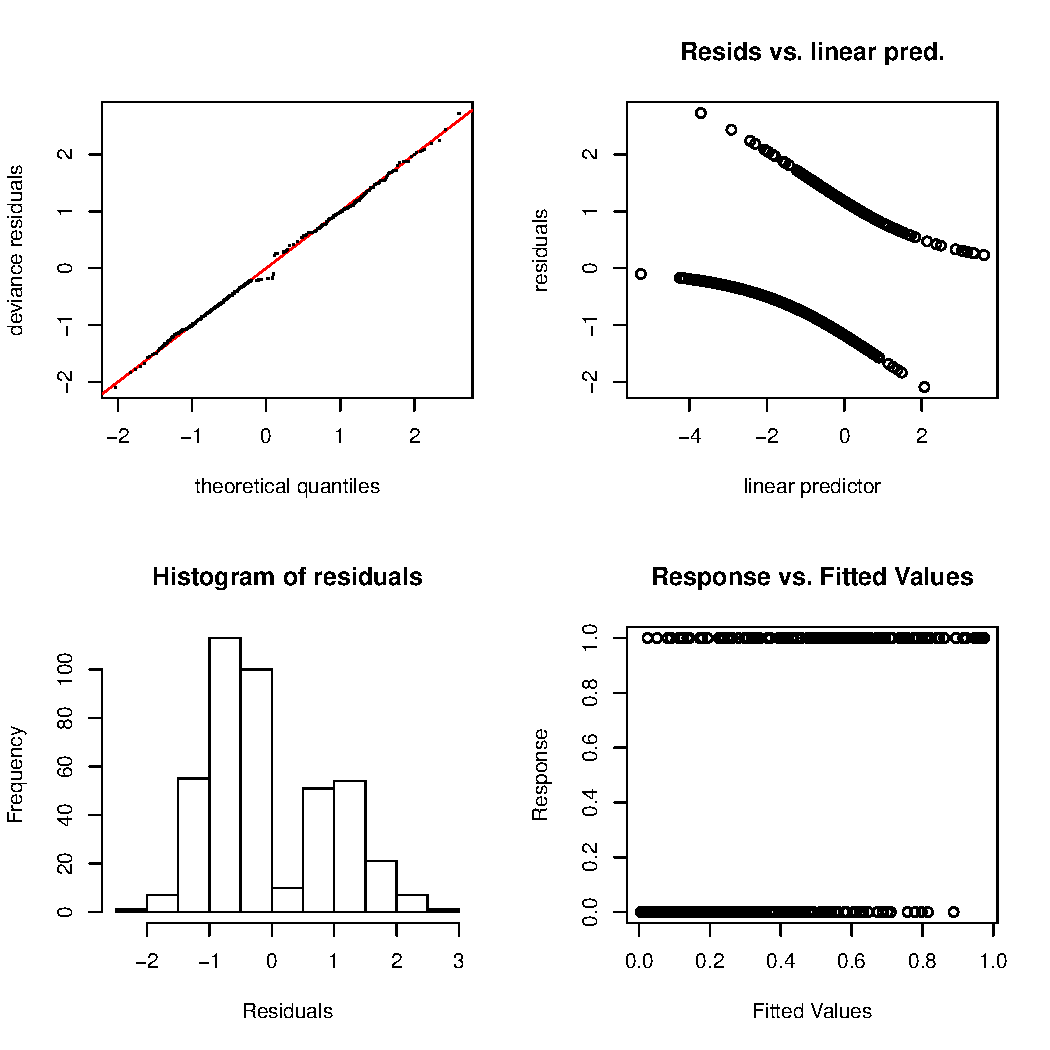
\includegraphics[width=\maxwidth]{figure/minimal-assumptionchecking1} 
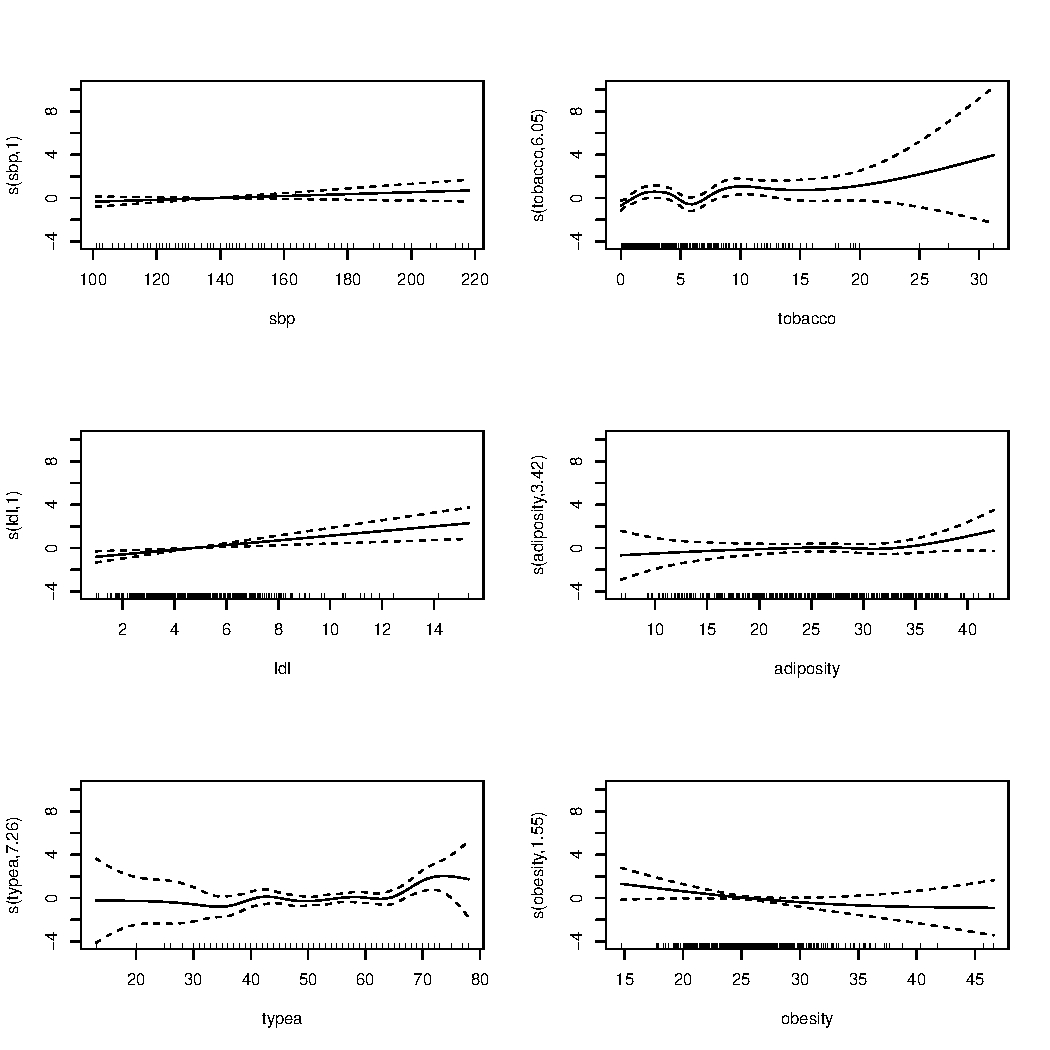
\includegraphics[width=\maxwidth]{figure/minimal-assumptionchecking2} 
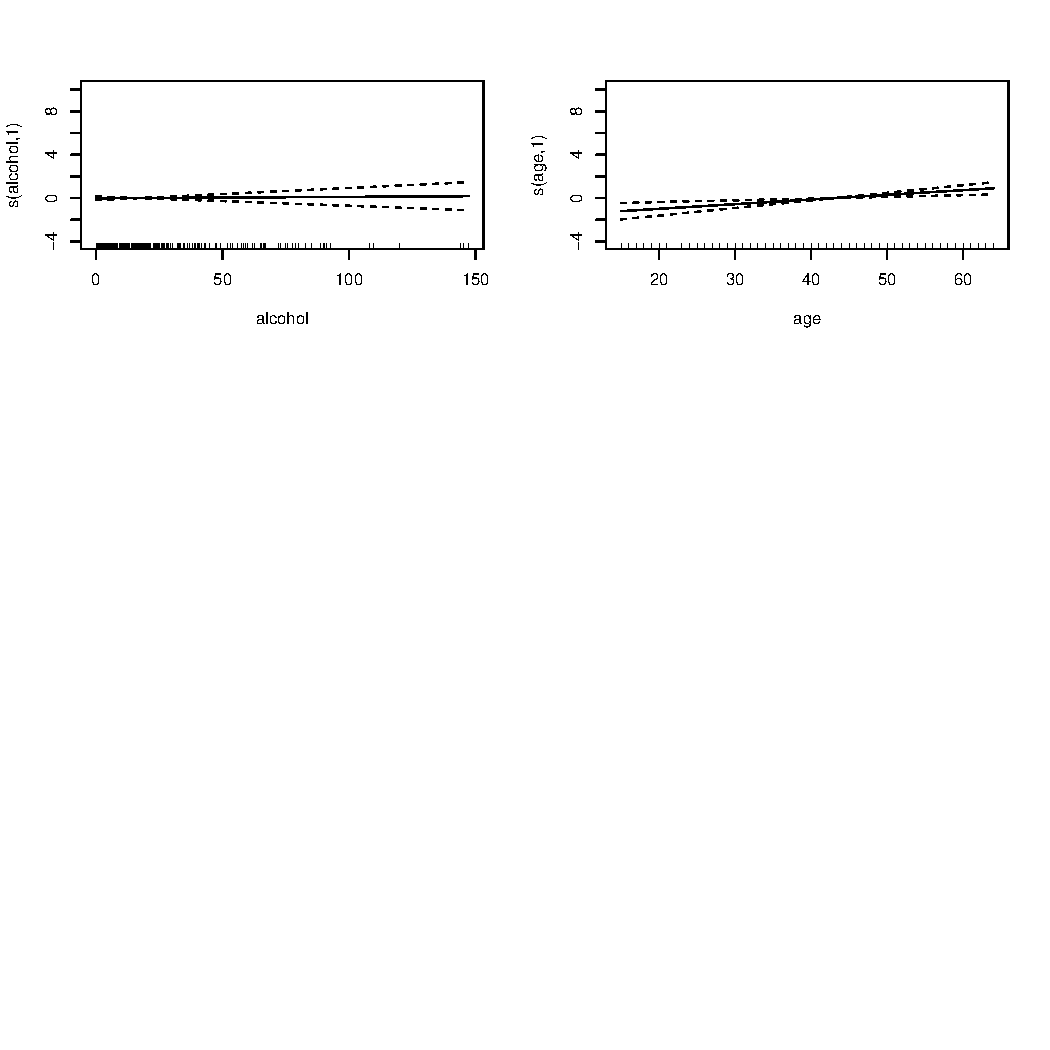
\includegraphics[width=\maxwidth]{figure/minimal-assumptionchecking3} 

}



\end{knitrout}

Looking at the residual, plot, we see that it is a little funky.  The qq norm plot indicates that there are a few issues with residuls being normally distributed, but since the m2 model still provides the best CV MSE, we will use it.

Our last step is to apply the model to the test data and round the results to 1 or zero:

\begin{knitrout}
\definecolor{shadecolor}{rgb}{0.969, 0.969, 0.969}\color{fgcolor}\begin{kframe}
\begin{alltt}
fitted_test_values <- \hlfunctioncall{predict.gam}(object = m2, newdata = SAH.test, se = TRUE, type = \hlstring{"response"})
\hlfunctioncall{round}(fitted_test_values$fit[1:42])
\end{alltt}
\begin{verbatim}
## 421 422 423 424 425 426 427 428 429 430 431 432 433 434 435 436 437 438 439 440 441 442 
##   1   1   0   0   0   1   0   0   0   0   0   0   1   0   0   1   0   0   0   0   0   0 
## 443 444 445 446 447 448 449 450 451 452 453 454 455 456 457 458 459 460 461 462 
##   0   0   0   1   0   1   0   1   1   1   0   0   0   0   0   0   0   0   0   1
\end{verbatim}
\end{kframe}
\end{knitrout}

\end{document}
